% Chapter 2

\chapter{Diseño del hardware y software}
\label{Chap:DisHard} % For referencing the chapter elsewhere, use \ref{Chapter2} 

%----------------------------------------------------------------------------------------

\section{Introducción}

En este capítulo se presenta información referente al funcionamiento general del sistema. Se divide en dos secciones: el hardware y el software, donde en cada uno se muestran diagramas o imágenes de funcionamiento, junto a una breve explicación.\\

En el diagrama de la figura~\ref{fig:null1} se muestra la relación existente entre una función a desempeñar y el dispositivo asociado.

\begin{figure}[ht]
\centering
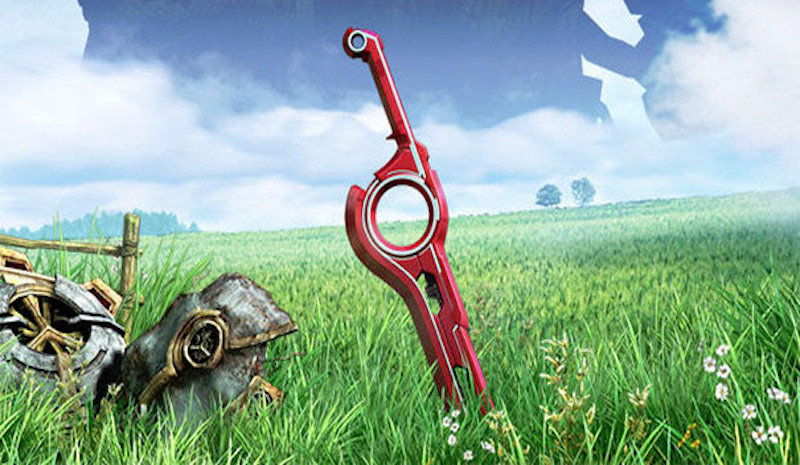
\includegraphics[scale=0.12]{Figures/null}
\caption[null.]{Null.\footnotemark}
\label{fig:null1}
\end{figure}

\footnotetext{null}

\section{Hardware}

\subsection{Prototipo}

El sistema cuenta con dos estaciones: una que es conocida como\textit{estación base} y es la encargada de ofrecer datos de corrección de las observaciones de GPS, y una estación móvil, cuyo posicionamiento se desea conocer. 

\subsection{Descripción de la estación base}

La estación base cuenta con dos componentes principales:

\begin{itemize}
\item GPS Ublox C94-M8P.
\item Comunicación inalámbrica.
\end{itemize}

En la memoria de la tarjeta Ublox C94-M8P de esta estación se encuentran las coordenadas de su posición actual (se pueden actualizar vía PC utilizando el Anexo de Configuración de los Dispositivos Ublox, adjunto a esta tesis).\\

Mediante la comunicación inalámbrica, los datos de posicionamiento necesarios para aplicar correcciones son enviadas a la tarjeta Ublox de la estación móvil, utilizando el protocolo RTCM3.

\subsection{Descripción de la estación móvil}

\subsubsection{Obtención de datos de GPS}

El diseño de los componentes de la estación móvil gira en torno a las capacidades y al diseño del GPS Ublox C94-M8P. De este dispositivo se tomarán dos datos importantes: \textbf{datos de posicionamiento de esta misma tarjeta}, ofrecidos por un \textbf{puerto microUSB}, y los \textbf{datos de corrección de posición} proporcionados por la estación base a través de comunicación inalámbrica, obtenidos por \textbf{protocolo RS232}, razón por la cual, en la tarjeta BeagleBone Black, son tomados el puerto USB y un puerto (dos pines) de comunicación serial.\\

\subsubsection{Visualización de resultados}

Para la visualización de los datos durante el funcionamiento del sistema, se dispone de una pantalla LCD 16x2 RGB conectada a pines de entrada/salida de uso general de la BeagleBone de la forma que muestra la siguiente figura~\ref{fig:null2}:

\begin{figure}[ht]
\centering
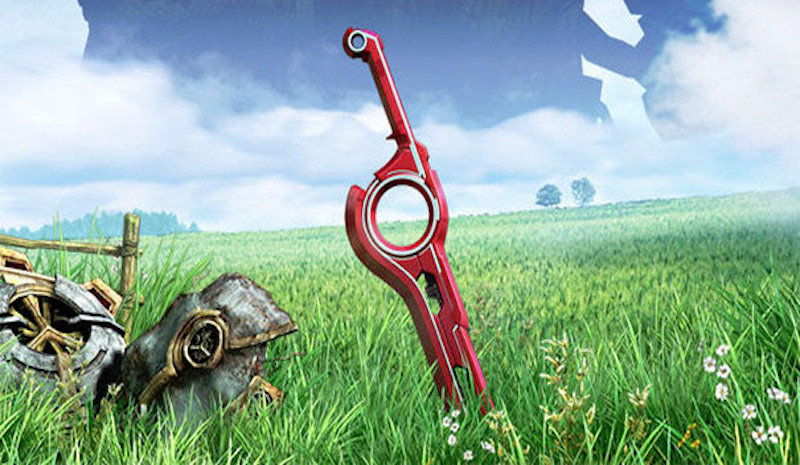
\includegraphics[scale=0.12]{Figures/null}
\caption[null.]{Null.\footnotemark}
\label{fig:null2}
\end{figure}

\footnotetext{null}

En la figura~\ref{fig:null3}, se puede observar dicha LCD proporcionando datos ya procesados de localización. 

\begin{figure}[ht]
\centering
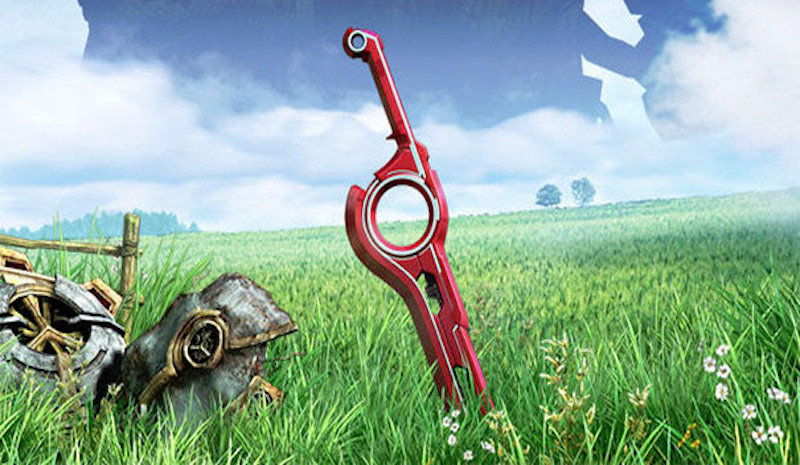
\includegraphics[scale=0.12]{Figures/null}
\caption[null.]{Null.\footnotemark}
\label{fig:null3}
\end{figure}

\footnotetext{null}

También, para un mejor control de estados del programa, se dispone de dos push buttons y un diodo LED conectados cada uno a pines de entrada/salida de uso general en la BeagleBone, tal y como muestra el circuito de la figura~\ref{fig:null4}.

\begin{figure}[ht]
\centering
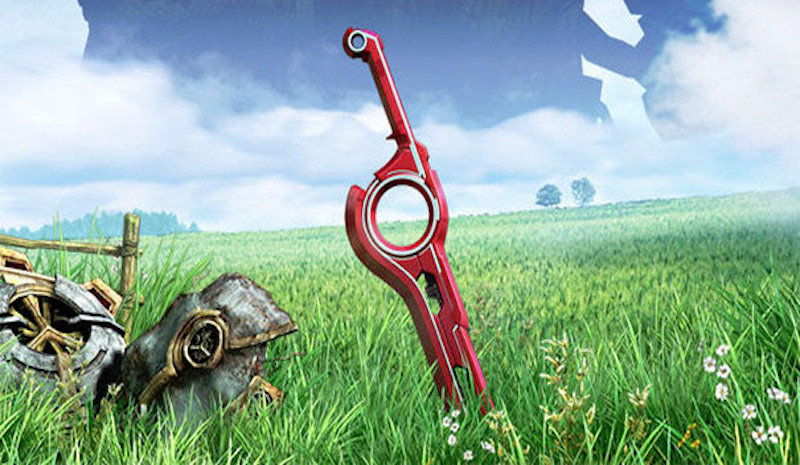
\includegraphics[scale=0.12]{Figures/null}
\caption[null.]{Null.\footnotemark}
\label{fig:null4}
\end{figure}

\section{Software}

En el apartado de software, se cuenta con dos conjuntos importantes de código: \textbf{RTKLIB} y bibliotecas para manejo de los pines de entrada/salida de uso general. Mediante estos últimos, fueron implementados los programas que controlan a los diversos periféricos de hardware conectados, incluido el GPS.

\subsection{RTKLIB}

Para una correcta implementación de RTKLIB\footnotemark en la BeagleBone Black, basada en arquitectura ARM, se pasó por distintas etapas:

\footnotetext{La versión utilizada es la beta 26 de RTKLIB en su versión 2.4.3, dado que es a partir de estas betas que se da soporte a los mensajes proporcionados por Ublox C94-M8P}

\begin{itemize}
\item \textbf{Configuración en Windows x86\_64:} Dadas las facilidades ofrecidas por RTKLIB en este sistema operativo (dos de ellas y las más importantes, el entorno gráfico y la cantidad de documentación) se decidió configurar el sistema primero bajo Windows. Mediante RTKNAVI, una aplicación de RTKLIB, se configuró el entorno para que reconociese los mensajes de GPS a través de USB, los distintos modos de funcionamiento, y cómo otorgaba los datos ya procesados, además de observación de geolocalización mediante un mapa al momento de la puesta en marcha.\\
\item \textbf{Hacer funcionar el sistema en GNU/Linux x86\_64:} Una vez funcionando RTKLIB en Windows, el objetivo de este punto es el de transportarse a un ambiente intermedio entre el dispositivo de destino y de donde se configuró inicialmente, sabiendo que todo el hardware estaba correctamente conectado y funcionando. Se usa ahora la aplicación RTKRCV que es la equivalente en entorno consola a RTKNAVI en Windows. Se realizaron los ajustes necesarios para hacer operativo el sistema, tales como indicar las rutas de obtención de información.\\

Una captura de pantalla de RTKRCV funcionando puede verse en la figura~\ref{fig:rtkrcv1}.

\begin{figure}[H]
\centering
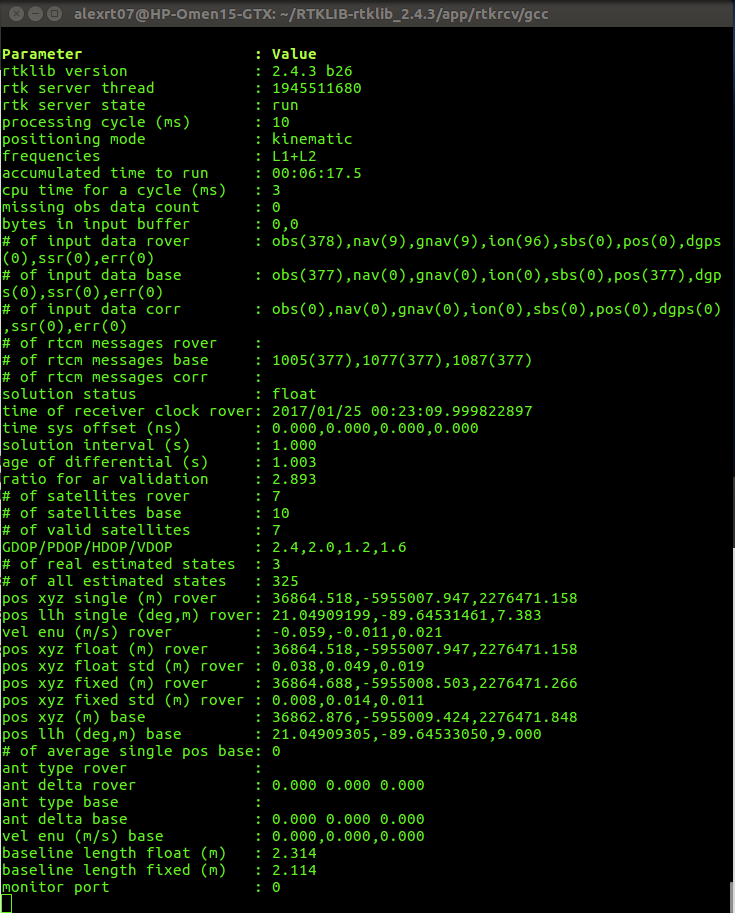
\includegraphics[scale=0.21]{Figures/LLH}
\caption[RTKRCV funcionando en GNU\_Linux PC.]{RTKRCV funcionando en GNU\_Linux PC.}
\label{fig:rtkrcv1}
\end{figure}

\item \textbf{Hacer funcionar el sistema en GNU/Linux ARM:} Una vez configurado correctamente para GNU/Linux en el punto anterior, sólo quedaba conectar todo a la microcomputadora BeagleBone y verificar que todo funcionase como en la PC. Los datos de salida de RTKLIB son ofrecidos vía socket y son recibidos a través de otro programa programado en C++ del que se hablará más adelante.
\end{itemize}

\subsection{Biblioteca BlackGPIO}

\subsubsection{Biblioteca GPS}

\subsubsection{Biblioteca LCD}

\section{Conclusión}

Lorem ipsum dolor...

En el capítulo siguiente...